\documentclass[16pt]{beamer}

\usepackage[utf8]{inputenc}
\usepackage[main=russian, english]{babel}
\usepackage{amssymb}
\usepackage{graphicx}

\usetheme{Warsaw}

\title[Конференция <<Ломоносовские чтения 2023>>]
        {Математическое моделирование движения руки и поведенческих движений}
\author[К. Ю. Егоров]
        {студент 2 курса магистратуры К. Ю. Егоров\\
        научный руководитель --- к.ф-м.н., доцент И. В. Востриков}
\institute{Кафедра системного анализа\\ ВМК МГУ}
\date{\today}

% Добавляем в панель навигации номер страницы
\setbeamertemplate{navigation symbols}{
        \insertslidenavigationsymbol
        \insertframenavigationsymbol
        \insertsubsectionnavigationsymbol
        \insertsectionnavigationsymbol
        \insertdocnavigationsymbol
        \insertbackfindforwardnavigationsymbol
        \hspace{1em}
        \usebeamerfont{footline}
        \insertframenumber /\inserttotalframenumber
        %
}

\begin{document}
    \begin{frame}
        \titlepage
    \end{frame}

    \begin{frame}{Введение}
        В работе приведен анализ движения руки человека:
        \begin{itemize}
            \item Построена математическая модель
            \item Поставлена задача оптимального управления для достижения целевого положения руки
            \item Предложен итеративный алгоритм синтеза управления
        \end{itemize}
        \vfill
        \begin{block}{Возможные применения}
            \begin{itemize}
                \item Разработка \textit{умных} протезов
                \item Разработка устройств для управления, корректирования движений людей с болезнями нервной системы
            \end{itemize}
            
        \end{block}
    \end{frame}

    \begin{frame}{Математическое моделирование}
        \centering{
            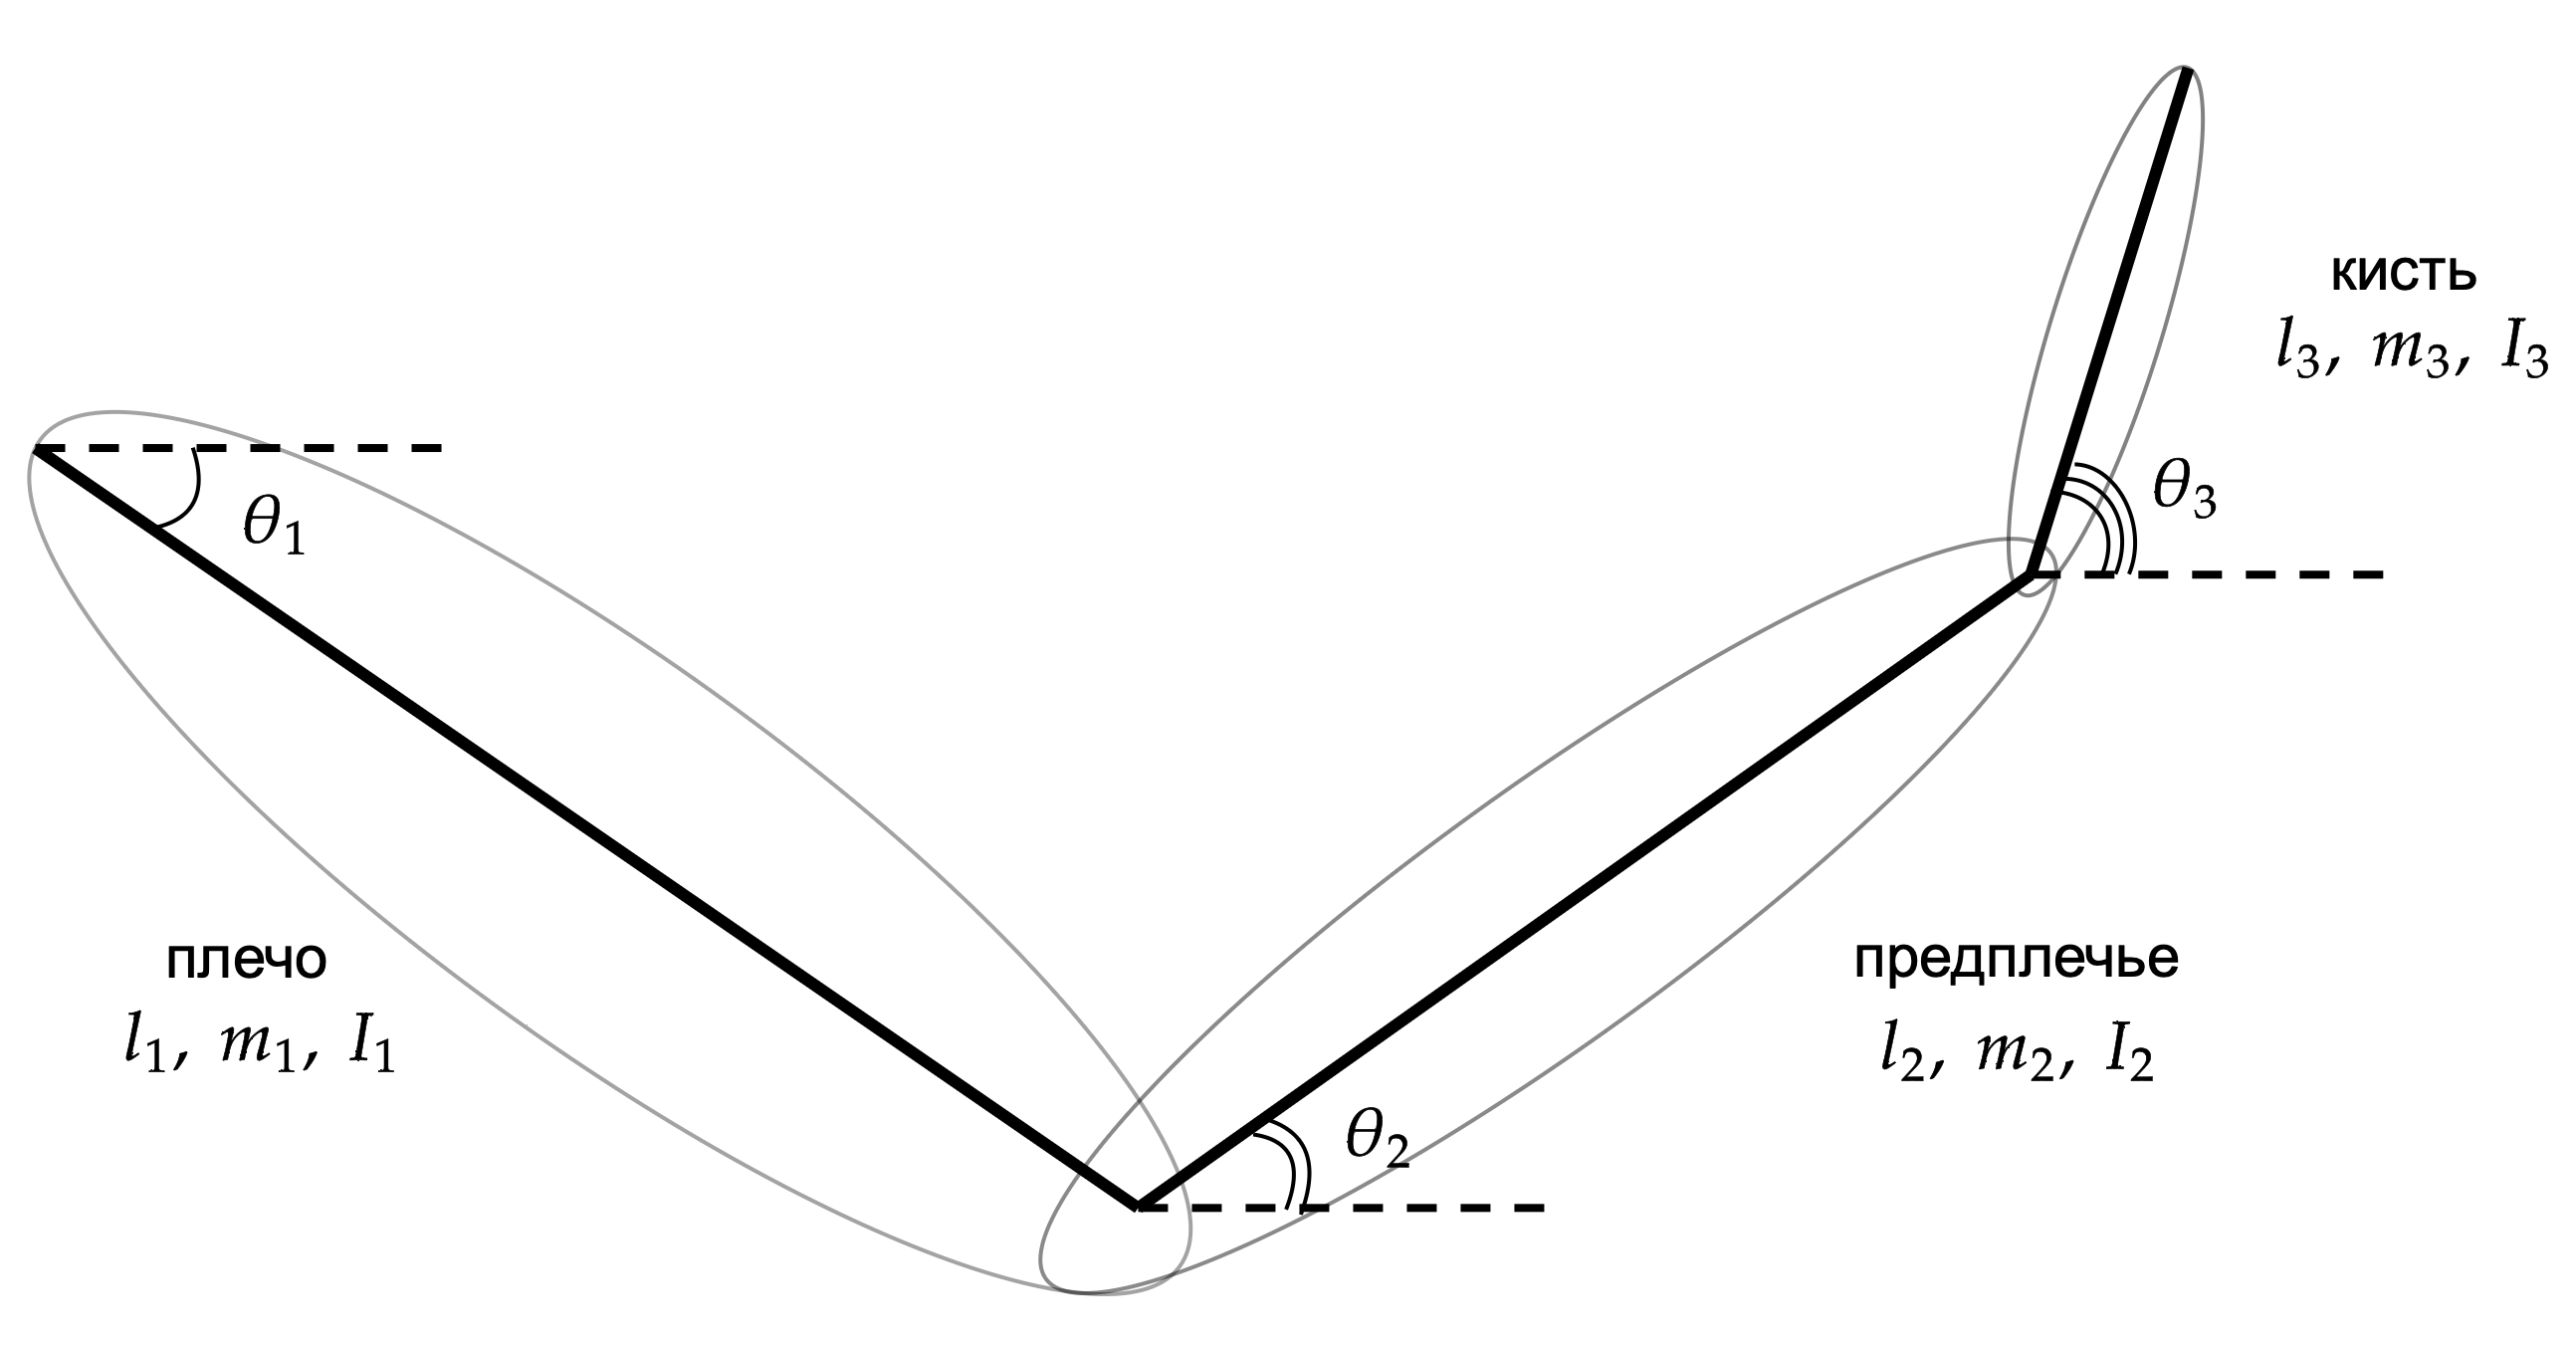
\includegraphics[width=0.8\textwidth]{diagram-20230405.png}
        }
        \begin{block}{Начальные данные}
            \begin{itemize}
                \item Рука --- 3-х сочленённый математический маятник.
                \item Известны длины $\ell_i$, массы $m_i$ и моменты инерции $I_i$.
                \item Фазовые переменные --- углы поворота сочленения $\theta_i$ относительно оси $Ox$. 
            \end{itemize}
        \end{block}
    \end{frame}

    \begin{frame}{Математическое моделирование}
        Метод Эйлера--Лагранжа
        $$
            \mathcal{L} = \Pi - K
            \;\Longrightarrow\;
            \tau_i
            =
              \frac{d}{dt}\left(\frac{\partial \mathcal{L}}{\partial \dot \theta_i}\right)
            - \frac{\partial \mathcal{L}}{\partial \theta_i},
        $$
        где $K$ и $\Pi$ --- общие кинетическая и потенциальная энергии системы.
        \vfill
        \begin{block}{Уравнение динамики}
            $$
                \tau = M(\theta)\ddot\theta + L(\theta, \dot\theta)
            $$
            \begin{itemize}
                \item $\tau_i$~--- момент силы, действующей на $i$-е сочленение
                \item $M(\theta)=M^{\mathrm{T}}(\theta)>0$~--- матрица инерции
                \item $L(\theta, \dot\theta)$~--- вектор центростремительных и корелисовых сил
            \end{itemize}
        \end{block}
    \end{frame}

    \begin{frame}{Математическое моделирование}
        \begin{figure}
            \includegraphics[width=0.8\textwidth]{discrete_pendulum.pdf}
            \caption{Траектория руки в свободном падении}
        \end{figure}
    \end{frame}

    \begin{frame}{Принцип оптимальности}
        \begin{itemize}
            \item Биологическое движение требует обработки большого количества информации
            \item Моторно-двигательная система как результат эволюции и обучения строит движение в соотвествии с принципом оптимальности
        \end{itemize}
        \vfill
        \begin{block}{Биологический принцип оптимальности}
            Выбираемые нервной системой схемы движения являются оптимальными для поставленной задачи.
        \end{block}
    \end{frame}

    \begin{frame}{Энергетические затраты}
        В работе [2] показано, что оптимизации проводится с целью уменьшения затрат энергии.
        \vfill
        \begin{block}{Формализация энергетических затрат [3]}
            $$
                \mbox{Затраты}\, = \int\limits_{t_{start}}^{t_{final}}\|\dot\tau\|^2\,dt
            $$
        \end{block}
    \end{frame}

    \begin{frame}{Задача достижения целевого положения}
        Введем $x = [\theta\;\dot\theta\;\tau]^{\mathrm{T}}$, тогда уравнение динамики примет вид
        $$
            \dot x = A(x) + Bu,\;
            \mbox{где}\,
            A(x) = \left[\begin{aligned}
                x_2 \\
                M^{-1}(x_1)(x_3 - L(x_1, x_2)) \\
                0
            \end{aligned}\right],
            B = \left[\begin{aligned}
                0 \\ 0 \\ 1
            \end{aligned}\right].
        $$
        Задано начальное положение:
        $$
            x(t_{start}) = x^{start}
        $$
        Задача минимизации функционала:
        $$
            J = w_1
            \underbrace{\langle x-x^{final}, x-x^{final} \rangle}_{Q^{final}(x)} + w_2 \int\limits_{t_{start}}^{t_{final}}\underbrace{\langle u, u\rangle}_{Q(x, u)}\,dt \longrightarrow \mathrm{min}
        $$
    \end{frame}

    \begin{frame}{Дискретизация задачи}
        Введем сетку по переменной $t = \{t_k\}_{k = 1}^{N+1}$ с шагом $\Delta t$ и дискретизируем задачу:
        $$
            \left\{
            \begin{aligned}
            &x^{k+1} = f(x^k, u^k) \\
            &x^0 = x^{start},
            \end{aligned}
            \right.
        $$
        где $f(x^k, u^k) = \Delta t [A(x^k) + Bu^k] + x^k$.
        $$
            J = Q^{N+1}(x^{N+1}) + \sum_{k=1}^{N} Q^{k}(x^k, u^k)\;\longrightarrow\;\mathrm{min},
        $$
        где $Q^{k}(x^k, u^k) = w_2 \Delta t Q(x^k, u^k)$, $Q^{N+1}(x^{N+1}) = w_1Q^{final}(x^{N+1})$.
    \end{frame}

    \begin{frame}{Дифференциальное динамическое программирование}
        \begin{block}{Идея метода}
            \begin{itemize}
                \item Берётся некоторое \textit{референсное} допустимое управление $u$ и соответствующая ей референсная траектория $x$
                \item Задача управления решается точно на каждой итерации алгоритма для коррекции референсного управления с целью снижения значения функции цены
                \item Используя информацию о градиенте гамильтониана $H$ на референсной траектории строится поправка вида
                $$
                    \Delta u = \eta \nabla_u H(u)
                $$
                \item Если решение не удовлетворяет заданной точности $\varepsilon$, получившееся управление берется в качестве референсного для следующей итерации алгоритма 
            \end{itemize}
        \end{block}
    \end{frame}

    \begin{frame}{Дифференциальное динамическое программирование}
        Пусть $(u, x)$~--- управление и соответствующая ему траектория на предыдущем шаге алгоритма. Рассмотрим Гамильтониан:
        $$
            H = Q_{N+1}(x^{N+1}) + \sum_{k=0}^N Q_k(x^k, u^k) + \sum_{k=0}^{N}\lambda_k^{\mathrm{T}}(x^{k+1} - f(x^k, u^k))
        $$
        \begin{block}{Необходимые условия оптимальности 1-ого порядка}
            \begin{align*}
                \frac{\partial H}{\partial \lambda_k} = x_{k+1} - f(x_k, u_k) &= 0 \\
                \frac{\partial H}{\partial x^k} = \frac{\partial Q_k}{\partial x}(x^k,u^k) - \frac{\partial f}{\partial x}^{\mathrm{T}}(x^k, u^k)\lambda_k + \lambda_{k-1} &= 0 \\
                \frac{\partial H}{\partial x^{N+1}} = \frac{\partial Q_{N+1}}{\partial x}(x^{N+1}) + \lambda_{N} &= 0 \\
                \frac{\partial H}{\partial u^k} = \frac{\partial Q_k}{\partial u}(x^k, u^k) - \frac{\partial f}{\partial u}^{\mathrm{T}}(x^k, u^k)\lambda_k &= 0
            \end{align*}
        \end{block}
    \end{frame}

    \begin{frame}{Дифференциальное динамическое программирование}
        \begin{enumerate}
            \item Рассчитать $\lambda_k$ для $k=N,\,N-1,\,\ldots,\,1$:
            
            $
                \begin{aligned}
                    &\lambda_N = - \frac{\partial Q_{N+1}}{\partial x}(x^{N+1})\\
                    &\lambda_{k-1} = \frac{\partial f}{\partial x^k}^{\mathrm{T}}(x^k, u^k)\lambda_k - \frac{\partial Q_k}{\partial x}(x^k, u^k)
                \end{aligned}
            $
            
            \item Рассчитать $\frac{\partial H}{\partial u_k}$ для $k=N,\,N-1,\,\ldots,\,1$:
            
            $
                \frac{\partial H}{\partial u_k} = \frac{\partial Q_k}{\partial u}(x^k, u^k) - \frac{\partial f}{\partial u}^{\mathrm{T}}(x^k, u^k)\lambda_k
            $

            \item Сделать поправку на исходную траекторию $u_k$, прибавив к ней поправку $\Delta u_k = -\eta\frac{\partial H}{\partial u_k}$,
            где коэффициент $\eta$ выбирается таким образом, чтобы получившееся управление было допустимым, то есть $u_k + \Delta u_k \in \mathcal{U}$.
            \item Остановить алгоритм в случае, если $\sum_{k=0}^n \left\| \frac{\partial H}{\partial u_k} \right\|^2 < \varepsilon$.
        \end{enumerate}
    \end{frame}

    \begin{frame}{Дифференциальное динамическое программирование}
        \begin{figure}
            \includegraphics[width=0.8\textwidth]{ddp_pendulum.pdf}
            \caption{Траектория руки, построенная методом ДДП.}
        \end{figure}
    \end{frame}

    \begin{frame}{Дифференциальное динамическое программирование}
        \begin{figure}
            \includegraphics[width=0.8\textwidth]{ddp_empty.pdf}
            \caption{Траектории схвата для итеративного алгоритма при нулевом начальном управлении $u^{ref}\equiv 0$. Показана каждая 3-я итерация.}
        \end{figure}
    \end{frame}
    
    \begin{frame}{Референсная траектория}
        \begin{block}{Мотивация}
            \begin{itemize}
                \item Градиентный метод сходится довольно долго
                \item Мы хотим выбрать начальное референсное управление таким образом, чтобы оно частично удовлетворяло условию задачи, с целью сократить число итераций алоритма
                \item Это управление должно \textit{быстро} строиться
                \item Оно должно быть допустимым для рассматриваемой задачи
            \end{itemize}
        \end{block}
    \end{frame}

    \begin{frame}{Референсная траектория}
        Приведем систему к линейной, заменой управления
        $$
            v = M^{-1}(x_1)(\tau - L(x_1, x_2))
        $$
        Тогда система примет вид:
        \begin{equation}\label{eq:linear}
            x^{k+1} =  \underbrace{\mathrm{diag}\{I,O\}}_{A_{ref}} x^{k} + \underbrace{\mathrm{diag}\{O, I\}}_{B_{ref}} v^{k}
        \end{equation}

        Решим для системы \eqref{eq:linear} задачу минимизации интегрально-квадратичного функционала:
        $$
            J^{ref} = \langle (x-x^{final}), T^{final}(x-x^{final}) \rangle + \sum_{k=1}^{N} \langle v^k, Tv^k \rangle \longrightarrow \mathrm{min}
        $$

        Получим референсное управление $u$ из соотношения
        $$
            \tau^k = M(x_1^k)v^k + L(x_1^k,x_2^k) \;\Longrightarrow\; u^{k} = \frac{\tau^{k+1} - \tau^{k}}{\Delta t}
        $$
    \end{frame}

    \begin{frame}{Референсная траектория}
        Метод динамического программирования даёт решение данной задачи:
        $$
            v^k_* = -[T + B_{ref}^{\mathrm{T}}P^kB_{ref}]^{-1}P^kB_{ref}A_{ref} x,
        $$
        где матрица $P^k$ может быть посчитана в обратном времени как решение уравнения Риккати:
        $$
            \begin{aligned}
                &P^{k-1} = A_{ref}^{\mathrm{T}} P^{k} A_{ref} - A_{ref}^{\mathrm{T}}P^kB_{ref}[T + B_{ref}^\mathrm{T}P^kB_{ref}]^{-1}B_{ref}^{\mathrm{T}}P^{k}A_{ref}
                \\
                &P^{N+1} = T^{final}
            \end{aligned}
        $$
        \begin{block}{Полученное управление}
            \begin{itemize}
                \item Считается за одну итерацию
                \item Минимизирует изменение углового ускорения, значит, допустимо
                \item Приводит нас к целевому положению, но ничего не говорит об энергии
            \end{itemize}
        \end{block}
    \end{frame}

    \begin{frame}{Референсная траектория}
        \begin{figure}
            \includegraphics[width=0.8\textwidth]{ddp_dummy.pdf}
            \caption{Траектории схвата для итеративного алгоритма при новом начальном управлении. Показана \textit{КАЖДАЯ} итерация.}
        \end{figure}
    \end{frame}

    \begin{frame}{Пример [Обход препятствий]}
        Добавим компонент в функцию цены:
        $$
            J_{\,\mbox{\small{преп}}} = w_3 \int_{t_{start}}^{t_{final}} \left(\| e_{\,\mbox{\small{схв}}} - e_{\,\mbox{\small{преп}}} \|^2 - r_{\,\mbox{\small{преп}}}\right)^{-2}\,dt,
        $$
        где
        \begin{itemize}
            \item $e_{\,\mbox{\small{схв}}}$ --- положение схвата
            \item $e_{\,\mbox{\small{преп}}}$ --- центр препятствия
            \item $r_{\,\mbox{\small{преп}}}$ --- радиус препятствия
        \end{itemize}
        \vfill
        Далее будем пользоваться алгоритмом.
    \end{frame}

    \begin{frame}{Пример [Обход препятствий]}
        \begin{figure}
            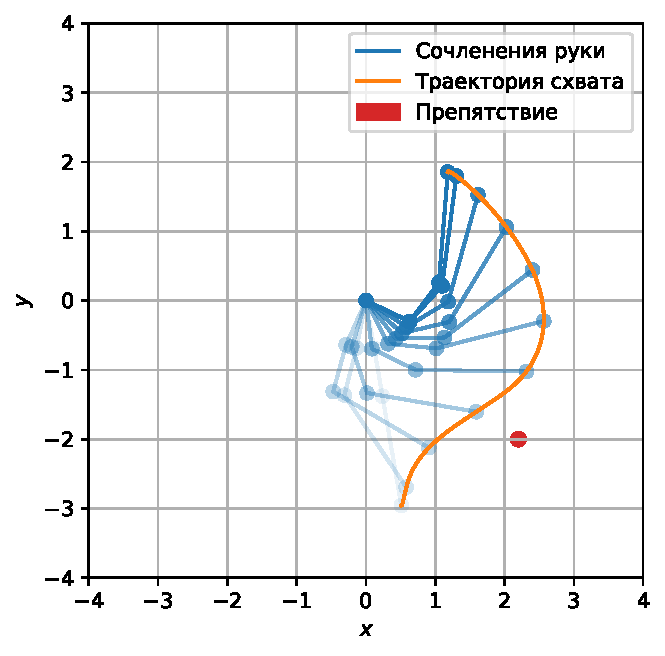
\includegraphics[width=0.49\textwidth]{obstacle_pendulum.pdf}
            \includegraphics[width=0.49\textwidth]{ddp_obstacle.pdf}
            \caption{Траектории руки и схвата для задачи обхода препятствия}
        \end{figure}
    \end{frame}

    \begin{frame}{Список литературы}
        \begin{enumerate}
            \item[1] Колюбин~С.\,А. Динамика робототехнических систем~// Учебное пособие. --- СПб.: Университет ИТМО, 2017.~--- 117 с.
            \item[2] E. Todorov, M. Jordan. Optimal feedback control as a theory of motor coordination~// Nature Neuroscience, Vol.5, No.11, 1226-1235, 2002.
            \item[3] Y. Uno, M. Kawato, R. Suzuki. Formation and control of optimal trajectory in human multijoint arm movement~--- minimum torque-change model~// Biological Cybernetics 61, 89-101, 1989.
            \item[4] B.D.O. Anderson, J.B. Moore. Optimal Control: Linear Quadratic Methods~// Prentice Hall, Upper Saddle River, 1990.
            \item[5] D. H. Jacobson. Differential dynamic programming methods for determining optimal control of non-linear systems~// University of London, 1967.
        \end{enumerate}
    \end{frame}

    \begin{frame}{Список литературы}
        \begin{enumerate}
            \item[6] E. Guechi, S. Bouzoualegh, Y. Zennir, S. Blažič. MPC Control and LQ Optimal Control of A Two-Link Robot Arm: A Comparative Study~// Machines 6, no. 3: 37, 2018.
            \item[7] A. Babazadeh, N. Sadati. Optimal control of multiple-arm robotic systems using gradient method~// IEEE Conference on Robotics, Automation and Mechatronics, Singapore, pp. 312-317 vol.1, 2004.
        \end{enumerate}
    \end{frame}
\end{document}

\usepackage{amsmath}  % Математические 
\usepackage{amssymb}  % формулы
\usepackage{graphicx}

% Show only current section (without subsection in the frame header)
\setbeamertemplate{headline}{%
  \leavevmode%
  \begin{beamercolorbox}[wd=\paperwidth,ht=2.5ex,dp=1.5ex]{section in head/foot}%
    %\hfill
    \hspace{1em}\strut\insertsectionhead\hspace{.5em}\mbox{}%
  \end{beamercolorbox}%
  %\begin{beamercolorbox}[wd=.5\paperwidth,ht=2.5ex,dp=1.5ex]{subsection in head/foot}%
  %  \mbox{}\hspace{.5em}\strut\insertsubsectionhead\hfill%
  %\end{beamercolorbox}%
}

\title[Магистерская диссертация]
        {Математическое моделирование движений руки, держащей предмет}
\author[К. Ю. Егоров]
        {студент 2 курса магистратуры К. Ю. Егоров\\
        научный руководитель --- к.ф-м.н., доцент И. В. Востриков}
\institute{Кафедра системного анализа\\ ВМК МГУ}
\date{26 апреля 2023}

\begin{document}
    \begin{frame}
        \titlepage
    \end{frame}

    \begin{frame}{Содержание}
        \tableofcontents
    \end{frame}


    \section{Построение математической модели}

    \begin{frame}{Математическое моделирование}
        \centering{
            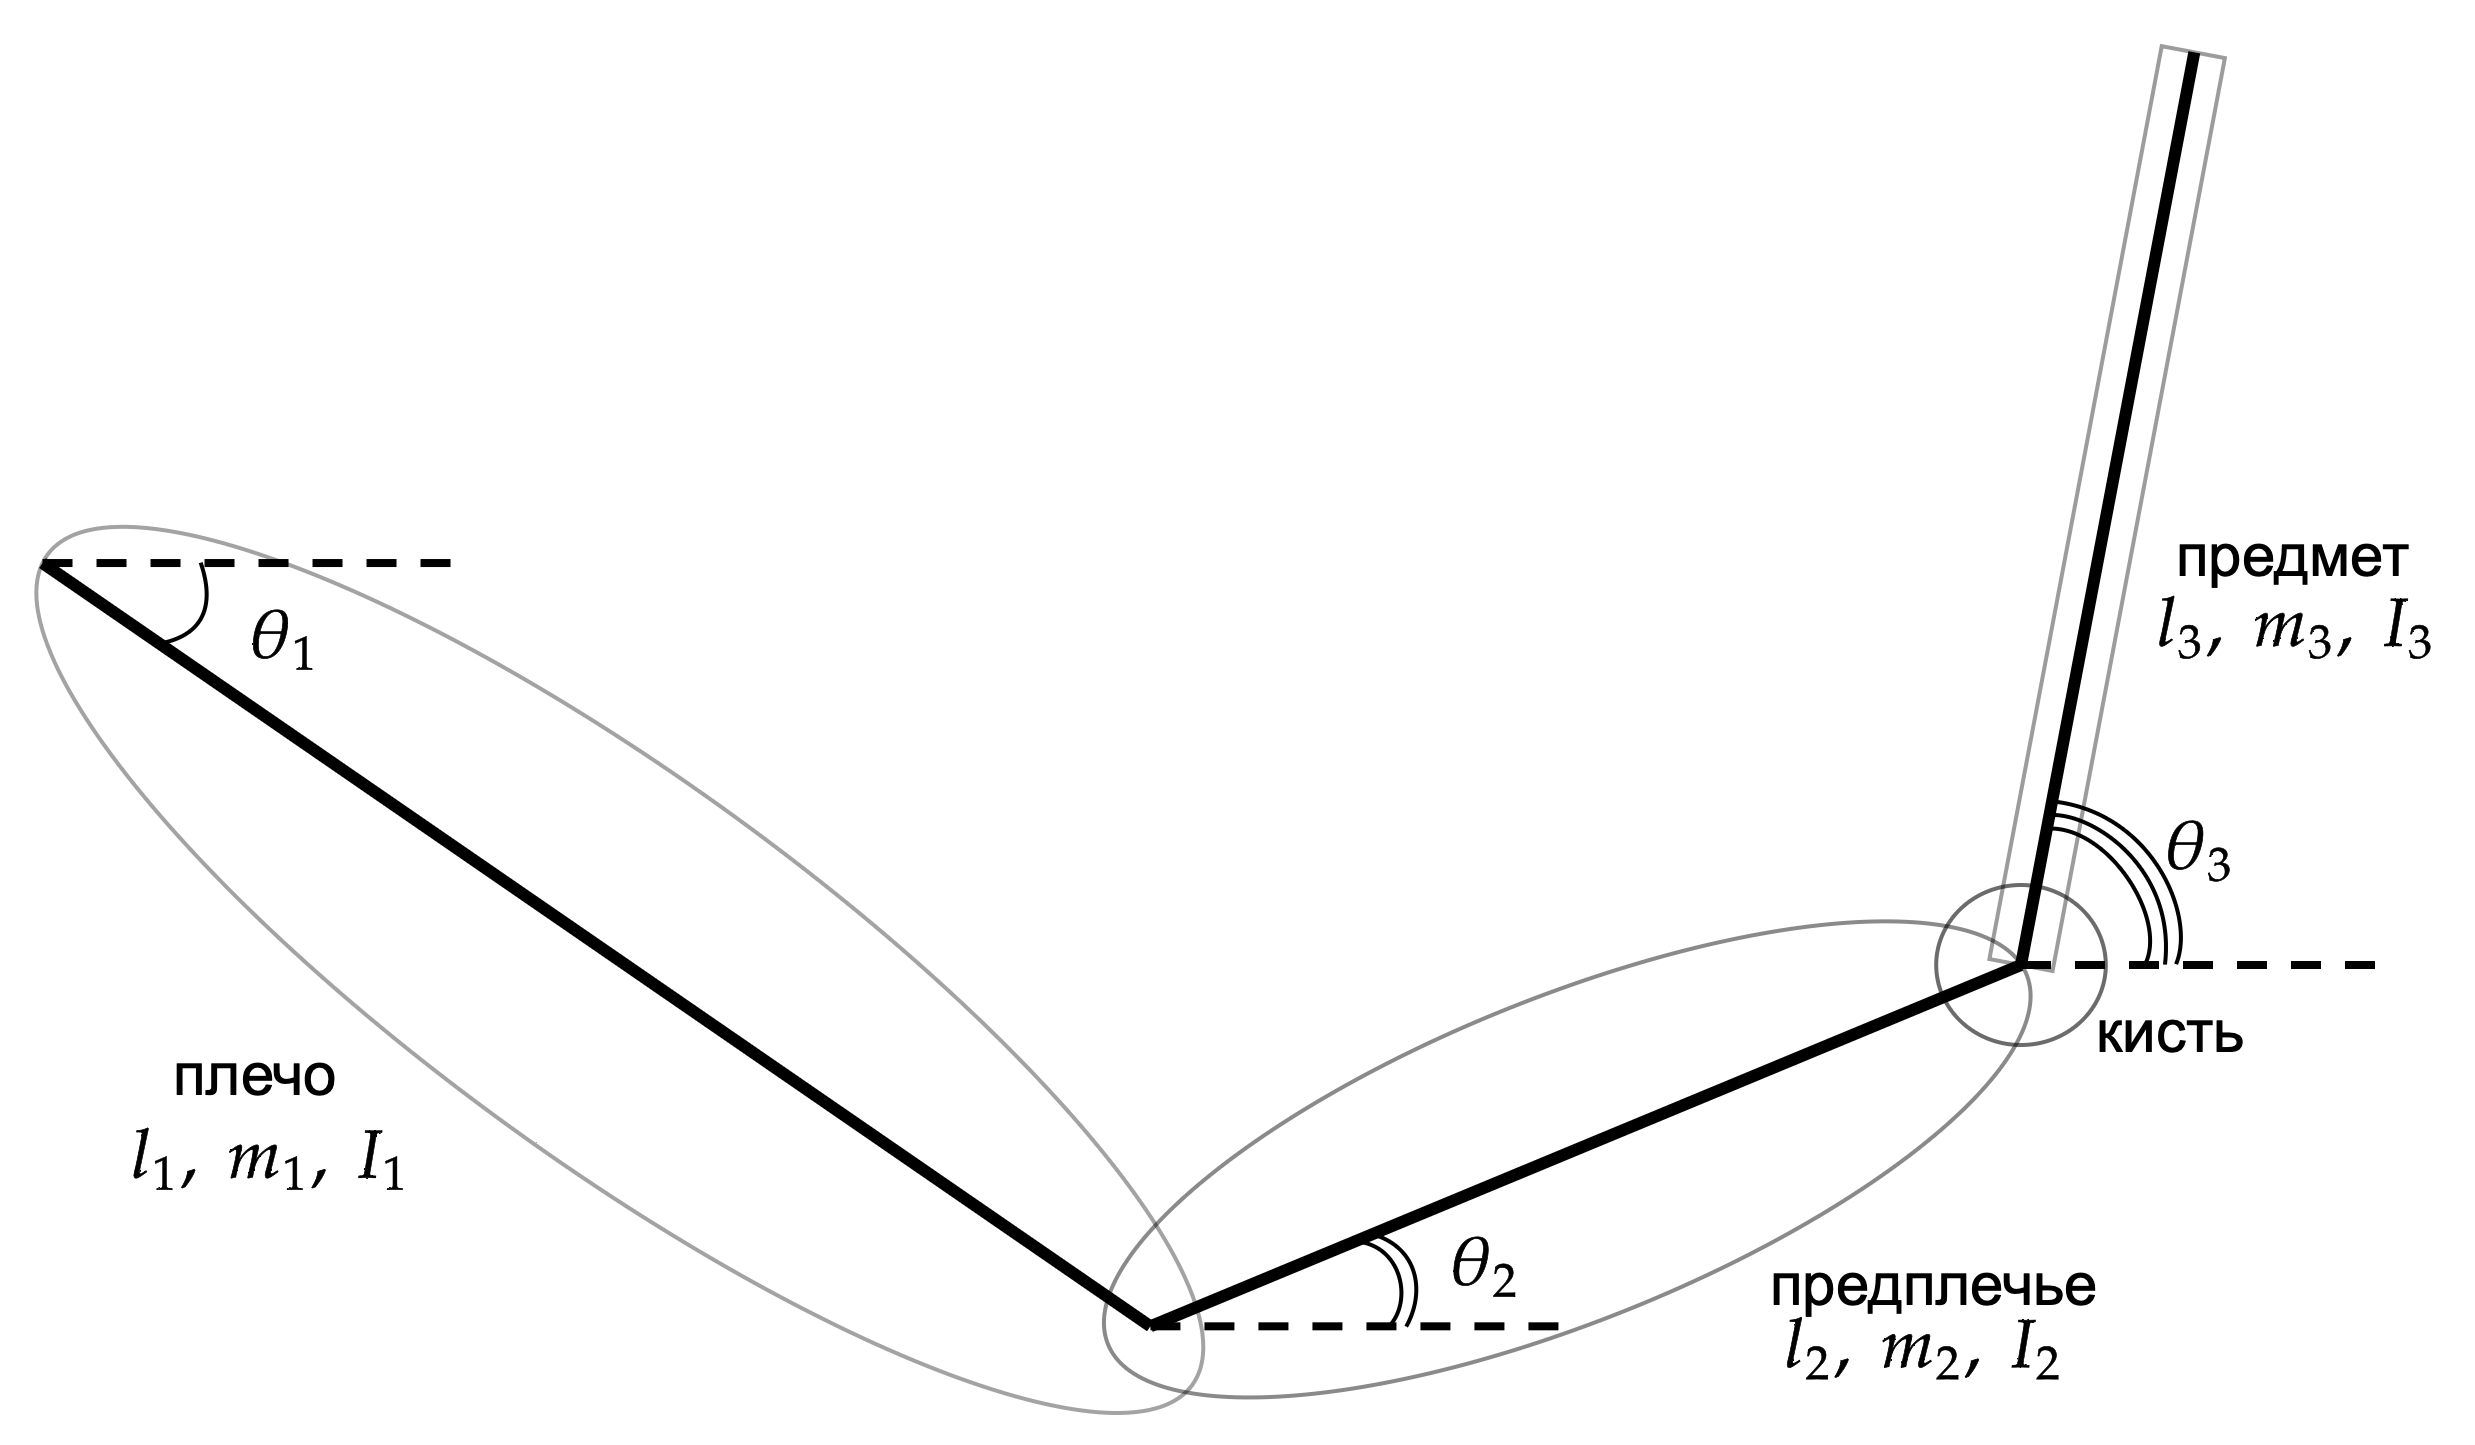
\includegraphics[width=0.7\textwidth]{img/arm.png}
        }
        \begin{block}{Начальные данные}
            \begin{itemize}
                \item Рука --- 3-х сочленённый математический маятник.
                \item Известны длины $\ell_i$, массы $m_i$ и моменты инерции $I_i$.
                \item Фазовые переменные --- углы поворота сочленения $\theta_i$ относительно оси $Ox$. 
            \end{itemize}
        \end{block}
    \end{frame}

    \begin{frame}{Уравнение динамики}
        Метод Эйлера--Лагранжа
        $$
            \mathcal{L} = \Pi - K
            \;\Longrightarrow\;
            \tau_i
            =
              \frac{d}{dt}\left(\frac{\partial \mathcal{L}}{\partial \dot \theta_i}\right)
            - \frac{\partial \mathcal{L}}{\partial \theta_i},
        $$
        где $K$ и $\Pi$ --- общие кинетическая и потенциальная энергии системы.
        \vfill
        \begin{block}{Уравнение динамики}
            $$
                \tau = M(\theta)\ddot\theta + L(\theta, \dot\theta)
            $$
            \begin{itemize}
                \item $\tau_i$~--- момент силы, действующей на $i$-е сочленение
                \item $M(\theta)=M^{\textnormal{T}}(\theta)>0$~--- матрица инерции
                \item $L(\theta, \dot\theta)$~--- вектор центростремительных и корелисовых сил
            \end{itemize}
        \end{block}
    \end{frame}

    \begin{frame}{Математическое моделирование}
        \begin{figure}
            \includegraphics[width=0.8\textwidth]{img/discrete_pendulum.pdf}
            \caption{Траектория руки в свободном падении}
        \end{figure}
    \end{frame}

    \begin{frame}{Принцип оптимальности}
        Моторно-двигательная система как результат эволюции и обучения строит движение в соотвествии с принципом оптимальности.
        \begin{block}{Биологический принцип оптимальности}
            Выбираемые нервной системой схемы движения являются оптимальными для поставленной задачи.
        \end{block}
        \vfill
        В работе [2] показано, что оптимизации проводится с целью уменьшения затрат энергии.
        \begin{block}{Формализация энергетических затрат [3]}
            $$
                \mbox{Затраты}\, = \int\limits_{t_{start}}^{t_{final}}\|\dot\tau\|^2\,dt
            $$
        \end{block}
    \end{frame}


    \section{Постановка задачи оптимального управления}

    \begin{frame}{Постановка задачи}
        Введем $x = [\theta\;\dot\theta\;\tau]^{\textnormal{T}}$, тогда уравнение динамики примет вид
        $$
            \dot x = A(x) + Bu,\;
            \mbox{где}\,
            A(x) = \left[\begin{aligned}
                x_2 \\
                M^{-1}(x_1)(x_3 - L(x_1, x_2)) \\
                O
            \end{aligned}\right],
            B = \left[\begin{aligned}
                0 \\ 0 \\ I
            \end{aligned}\right].
        $$
        Задано начальное положение:
        $$
            x(t_{\textnormal{start}}) = x^{\textnormal{start}}
        $$
        Задача минимизации функционала:
        $$
            J
            =
            q_{\textnormal{терм.}}(x^{\textnormal{final}})
            +
            w_1\int_{t_{\textnormal{start}}}^{t_{\textnormal{final}}} q_{\textnormal{фаз.}}(x)\,dt
            +
            w_2\int_{t_{\textnormal{start}}}^{t_{\textnormal{final}}} \| u \|^2 \,dt
            \longrightarrow 
            \textnormal{min},
        $$
        где $q_{\textnormal{терм.}}$, $q_{\textnormal{фаз.}}$ выбираются исходя из конкретной постановки задачи.
    \end{frame}

    \begin{frame}{Дискретный вариант задачи}
        Введем сетку по переменной $t = \{t_k\}_{k = 1}^{N+1}$ с шагом $\Delta t$, тогда
        $$
            \left\{
            \begin{aligned}
            &x^{k+1} = f(x^k, u^k) \\
            &x^0 = x^{start},
            \end{aligned}
            \right.
        $$
        где $f(x^k, u^k) = \Delta t [A(x^k) + Bu^k] + x^k$.
        $$
            J
            =
            q^{N+1}(x^{N+1})
            +
            \sum_{k=1}^{N} q^{k}(x^k)
            +
            \sum_{k=1}^{N} r^{k}(u^k)
            \;\longrightarrow\;\textnormal{min},
        $$
        $q^{N+1}(x) = q_{\textnormal{терм.}}(x)$, $q^{k}(x) = w_1 \Delta t q_{\textnormal{фаз.}}(x)$, $r^k(u) = w_2 \Delta t \| u \|^2$.
    \end{frame}


    \section{Алгоритм синтеза управления}

    \begin{frame}{Алгоритм синтеза управления}
        \begin{block}{Идея метода}
            \begin{enumerate}
                \item Пусть на $k$ шаге алгоритма дано \textit{референсное} управление $\bar u$ и соответствующая ему траектория $\bar x$.
                \item Вдоль траектории линеаризуем систему, квадратично аппроксимируем функционал качества.
                \item Построим оптимальную поправку на управление {\centering $\delta u = \delta u(\bar x, \bar u).$}
                \item Если поправка выходит за допустимую область, то есть $\bar u^k + \delta u^k \notin \mathcal{U}^k$, то берем в качестве поправки $\eta\delta u^k$ такую, что {\centering $\bar u^k + \eta\delta u^k \in \partial \mathcal{U}^k.$}
                \item Если мы не достигли требуемой точности, то есть $|J(\bar u) - J(\bar u + \delta u)| \geqslant \varepsilon$, повторяем действия с новым референсным управлением.
            \end{enumerate}
        \end{block}
    \end{frame}

    \begin{frame}{Аппроксимированная задача}
        Допустим мы имеем некоторое референсное управление~$\bar u$ и соответствующую ему референсную траекторию~$\bar x$.
        \begin{equation}\label{eq:ref-system}
            \left\{\begin{aligned}
                &\delta x^{k+1} = f_x^k \delta x + f_u^k \delta u \\
                &\delta x^0 = 0.
            \end{aligned}\right.
        \end{equation}
        \begin{multline}\label{eq:ref-cost}
            J = q^{N+1} + q_x^{N+1}\tilde x^{N+1} + \frac{1}{2}\langle \tilde x^{N+1}, q_{xx}^{N+1}\tilde x^{N+1} \rangle
            + \\ +
            \sum_{k=1}^{N}\left[ q^{k} + q_x^{k}\tilde x^{k} + \frac{1}{2}\langle \tilde x^{k}, q_{xx}^{k}\tilde x^{k} \rangle \right]
            + \\ +
            \sum_{k=1}^{N}\left[ r^{k} + r_u^{k}\tilde u^{k} + \frac{1}{2}\langle \tilde u^{k}, r_{uu}^{k}\tilde u^{k} \rangle \right],
        \end{multline}
        где $\tilde x^k = \bar x^k + \delta x^k$, $\tilde u^k = \bar u^k + \delta u^k$.
    \end{frame}

    \begin{frame}{Синтез управления}
        \begin{block}{Теорема [Об оптимальной поправке]}
            Оптимальная поправка $\delta u$ для задачи~\eqref{eq:ref-system}-\eqref{eq:ref-cost} вычисляется как
            \begin{equation*}
                \delta u^k = - (r^k_{uu} + (f^k_u)^{\textnormal{T}} S_{k+1} f^k_u)^{-1} ((f^k_u)^{\textnormal{T}} S_{k+1} f^k_u \delta x + v^{k+1} + r^k_u),
            \end{equation*}
            где $S_k$ и $v^{k}$ высчитываются в обратном времени как
            \begin{equation*}
                    S_k = q^k_{xx} + (f^k_x)^{\textnormal{T}} S_{k+1} (I + f^k_u (r^k_{uu})^{-1} (f^k_u)^{\textnormal{T}} S_{k+1})^{-1} f_x^k,
            \end{equation*}
            \begin{multline*}
                v^k = (f^k_x)^{\textnormal{T}} S_{k+1} ( I + f^k_u (r^k_{uu})^{-1} (f^k_u)^{\textnormal{T}} S_{k+1})^{-1}
                \cdot \\ \cdot
                (-f^k_u (r^k_{uu})^{-1} (f^k_u)^{\textnormal{T}} v^{k+1} + f^k_u (r^k_{uu})^{-1} r^k_u) + (f^k_x)^{\textnormal{T}} v^{k+1} + q^k_x
            \end{multline*}
            с граничными условиями
            \begin{equation*}
                    S_{N+1} = q^{N+1}_{xx},
                    \quad
                    v^{N+1} = q^{N+1}_{x}.
            \end{equation*}
        \end{block}
    \end{frame}
    
    \begin{frame}{Пример: Целевое состояние}
        $$
            q_{\textnormal{терм.}}(x) = \| x - x^{\textnormal{final}}\|^2
        $$
        \begin{figure}
            \centering{
                \includegraphics[width=0.45\textwidth]{img/ddp_pendulum.pdf}
                \includegraphics[width=0.45\textwidth]{img/ddp_empty.pdf}
            }
            \caption{Траектории руки и схвата для задачи при нулевом начальном управлении $\bar u \equiv 0$. Показана каждая 3-я итерация алгоритма.}
        \end{figure}
    \end{frame}


    \section{Выбор начальной траектории алгоритма}

    \begin{frame}{Выбор начальной траектории}
        \begin{block}{Мотивация}
            Предложенный метод сходится медленно. Построим начальное референсное управление $\bar u$ так, чтобы:
            \begin{itemize}
                \item Оно удовлетворяло терминальному условию;
                \item Оно \textit{быстро} строилось;
                \item Оно было допустимо для рассматриваемой задачи.
            \end{itemize}
        \end{block}
    \end{frame}

    \begin{frame}{Референсная траектория}
        Приведем систему к линейной, заменой управления
        $$
            v = M^{-1}(x_1)(\tau - L(x_1, x_2))
        $$
        Тогда система примет вид:
        \begin{equation}\label{eq:linear}
            x^{k+1} =  \underbrace{\textnormal{diag}\{I,O\}}_{A} x^{k} + \underbrace{\textnormal{diag}\{O, I\}}_{B} v^{k}
        \end{equation}

        Выберем $x^{\textnormal{final}} \in \textnormal{Argmin}_{x} q^{N+1}(x)$ и решим задачу минимизации

        \begin{equation}\label{eq:linear-cost}
            J = \| x-x^{\textnormal{final}} \|^2 + w \sum_{k=1}^{N} \| v^k \|^2 \longrightarrow \textnormal{min}
        \end{equation}

        Получим референсное управление $u$ из соотношения
        $$
            \tau^k = M(x_1^k)v^k_* + L(x_1^k,x_2^k) \;\Longrightarrow\; u^{k} = \frac{\tau^{k+1} - \tau^{k}}{\Delta t}
        $$
    \end{frame}

    \begin{frame}{Референсная траектория}
        Метод динамического программирования даёт решение задачи.
        \vfill
        \begin{block}{Утверждение}
            Оптимальное управление $v_*$ задачи \eqref{eq:linear}-\eqref{eq:linear-cost} высчитывается как
            $$
                v^k_* = -[wI + B^{\textnormal{T}}P^kB]^{-1} P^k B A x,
            $$
            где матрица $P^k$ может быть посчитана в обратном времени как решение уравнения Риккати
            $$
                \begin{aligned}
                    &P^{k-1} = A^{\textnormal{T}} P^{k} A - A^{\textnormal{T}} P^k B [wI + B^{\textnormal{T}} P^k B]^{-1} B^{\textnormal{T}} P^{k} A
                    \\
                    &P^{N+1} = I
                \end{aligned}
            $$
        \end{block}
    \end{frame}

    \begin{frame}{Пример: целевое состояние}
        $$
            q_{\textnormal{терм.}}(x) = \| x - x^{\textnormal{final}}\|^2
        $$
        \begin{figure}
            \centering{
                \includegraphics[width=0.45\textwidth]{img/ddp_pendulum.pdf}
                \includegraphics[width=0.45\textwidth]{img/ddp_dummy.pdf}
            }
            \caption{Траектории руки и схвата для задачи при новом начальном управлении. Показана \textit{КАЖДАЯ} итерация алгоритма.}
        \end{figure}
    \end{frame}


    \section{Применение в классических задачах}

    \begin{frame}{Задача: обход препятствия}
        $$
            \begin{aligned}
            & q_{\textnormal{терм.}}(x) = \| x - x^{\textnormal{final}}\|^2
            \\
            & q_{\textnormal{фаз.}}(x) = \left(\| e_{\textnormal{cхват}}(x) - e_{\textnormal{препят}}\|^2 - r_{\textnormal{препят}}\right)^2
            \end{aligned}
        $$
        \begin{figure}
            \centering{
                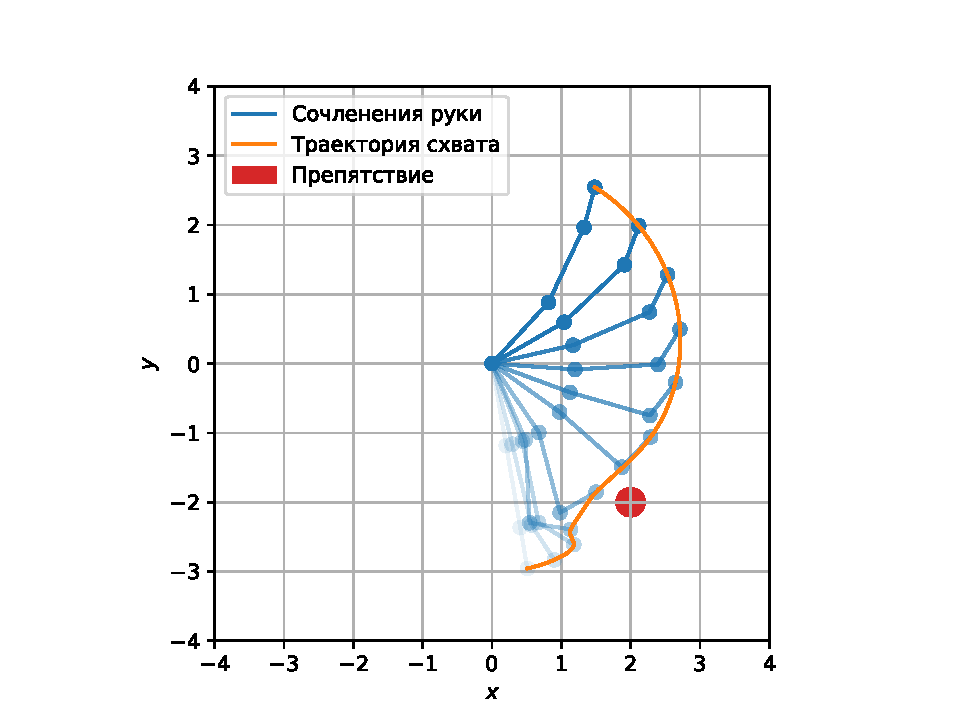
\includegraphics[width=0.45\textwidth]{img/obstacle_pendulum}
                \includegraphics[width=0.45\textwidth]{img/ddp_obstacle}
            }
            \caption{Траектории руки и схвата для задачи.}
        \end{figure}
    \end{frame}

    \begin{frame}{Задача: целевое положение схвата}
        $$
            q_{\textnormal{терм.}}(x) = \| e_{\textnormal{схват}}(x) - e^{\textnormal{final}}\|^2
        $$
        \begin{figure}
            \centering{
                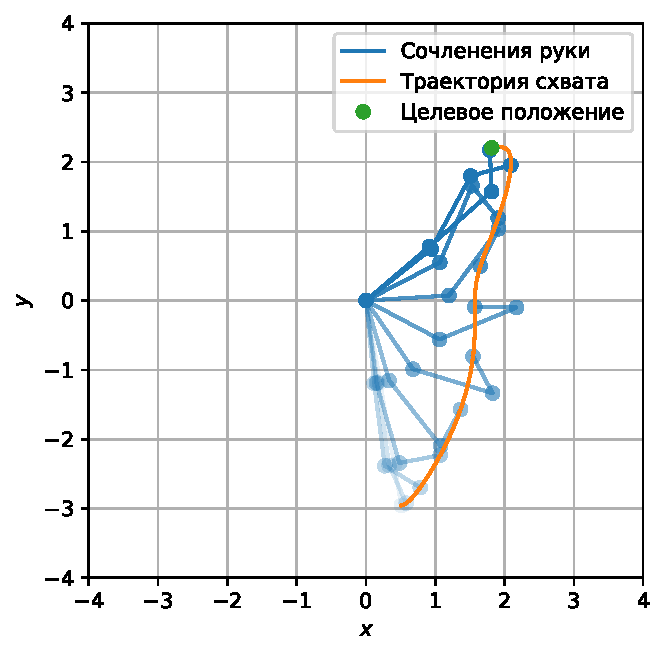
\includegraphics[width=0.45\textwidth]{img/reaching_pendulum}
                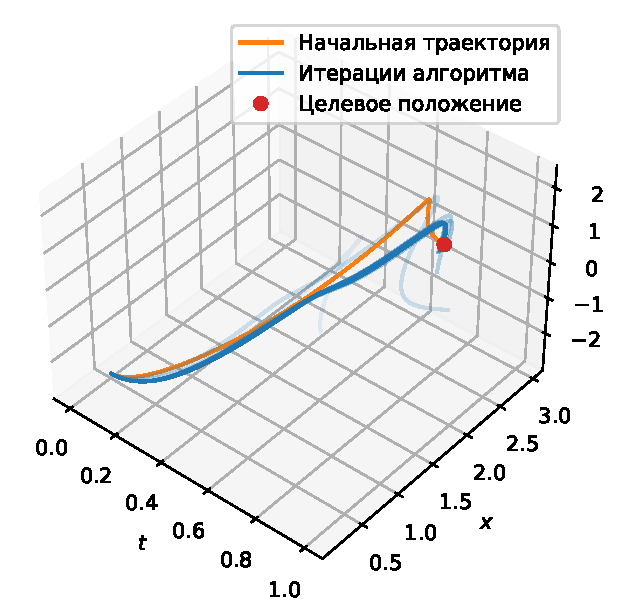
\includegraphics[width=0.45\textwidth]{img/ddp_reaching}
            }
            \caption{Траектории руки и схвата для задачи.}
        \end{figure}
    \end{frame}

    \begin{frame}{Задача: целевое положение схвата}
        $$
            \begin{aligned}
            & q_{\textnormal{терм.}}(x) = \| e_{\textnormal{схват}}(x) - e^{\textnormal{final}}\|^2
            \\
            & q_{\textnormal{фаз.}}(x) = \Sigma_{i=2}^{3} (x_i - x_{i-1})^2
            \end{aligned}
        $$
        \begin{figure}
            \centering{
                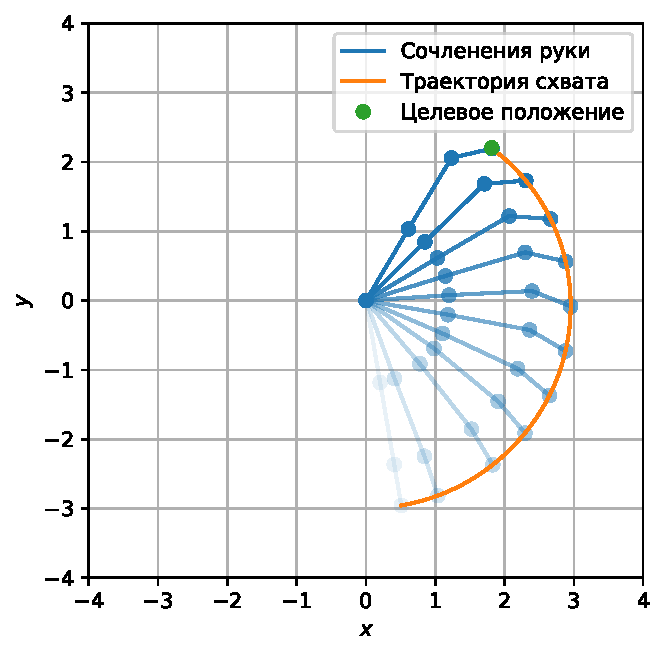
\includegraphics[width=0.45\textwidth]{img/reaching_phase_pendulum}
                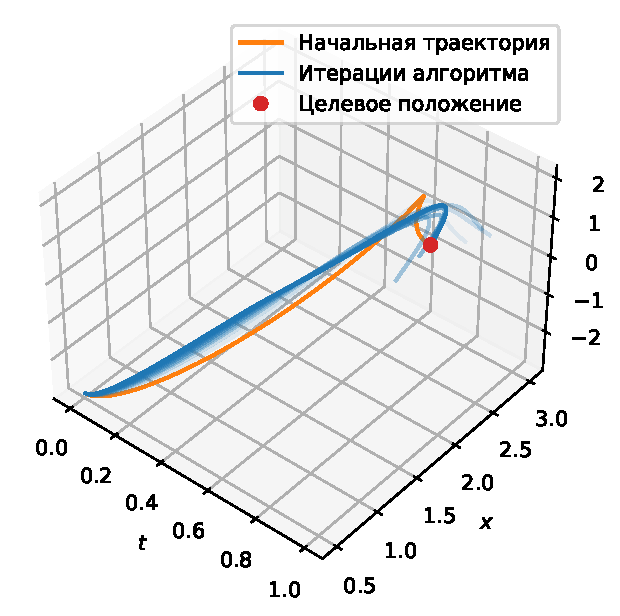
\includegraphics[width=0.45\textwidth]{img/ddp_reaching_phase}
            }
            \caption{Траектории руки и схвата для задачи.}
        \end{figure}
    \end{frame}

    \section{Литература}
    \begin{frame}{Доклады}
        \begin{itemize}
            \item Егоров К. Ю., Востриков И. В. Математическое моделирование движения руки и поведенческих движений // Доклад науч. конф. <<Ломоносовские чтения>> (Москва, 4-14 апреля 2023).
        \end{itemize}
    \end{frame}

    \begin{frame}{Список литературы}
        \begin{enumerate}
            \item[1] Колюбин~С.\,А. Динамика робототехнических систем~// Учебное пособие. --- СПб.: Университет ИТМО, 2017.~--- 117 с.
            \item[2] E. Todorov, M. Jordan. Optimal feedback control as a theory of motor coordination~// Nature Neuroscience, Vol.5, No.11, 1226-1235, 2002.
            \item[3] Y. Uno, M. Kawato, R. Suzuki. Formation and control of optimal trajectory in human multijoint arm movement~--- minimum torque-change model~// Biological Cybernetics 61, 89-101, 1989.
            \item[4] B.D.O. Anderson, J.B. Moore. Optimal Control: Linear Quadratic Methods~// Prentice Hall, Upper Saddle River, 1990.
            \item[5] D. H. Jacobson. Differential dynamic programming methods for determining optimal control of non-linear systems~// University of London, 1967.
        \end{enumerate}
    \end{frame}

    \begin{frame}{Список литературы}
        \begin{enumerate}
            \item[6] E. Guechi, S. Bouzoualegh, Y. Zennir, S. Blažič. MPC Control and LQ Optimal Control of A Two-Link Robot Arm: A Comparative Study~// Machines 6, no. 3: 37, 2018.
            \item[7] A. Babazadeh, N. Sadati. Optimal control of multiple-arm robotic systems using gradient method~// IEEE Conference on Robotics, Automation and Mechatronics, Singapore, pp. 312-317 vol.1, 2004.
        \end{enumerate}
    \end{frame}
\end{document}